\begin{figure}[htbp]
\centering
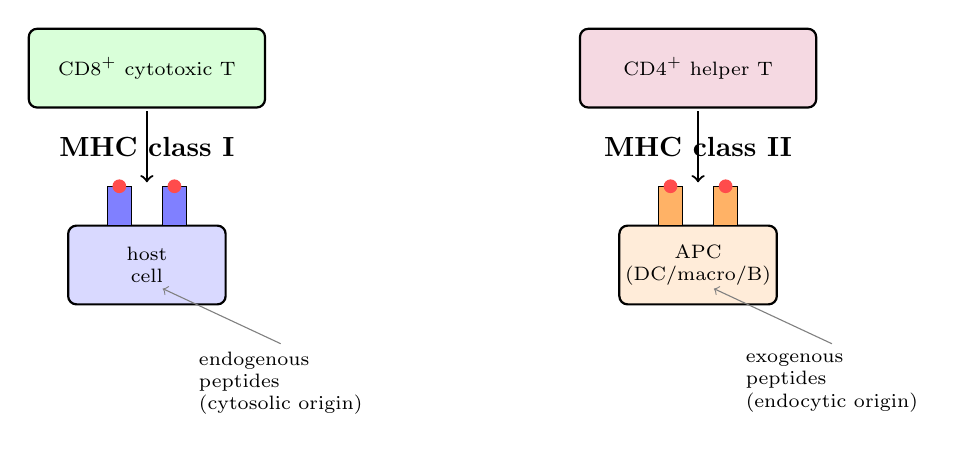
\begin{tikzpicture}[scale=1.0, every node/.style={font=\small}]
  % MHC class I panel
  \begin{scope}
    \node[font=\bfseries] at (2.5,4.5) {MHC class I};
    \draw[thick, fill=blue!15, rounded corners=3pt] (1.5,2.5) rectangle (3.5,3.5);
    \node[align=center, font=\scriptsize] at (2.5,3.0) {host\\cell};
    % MHC I on surface
    \draw[fill=blue!50] (2.0,3.5) -- (2.0,4.0) -- (2.3,4.0) -- (2.3,3.5) -- cycle;
    \draw[fill=blue!50] (2.7,3.5) -- (2.7,4.0) -- (3.0,4.0) -- (3.0,3.5) -- cycle;
    % Peptide on MHC I
    \filldraw[red!70] (2.15,4.0) circle (0.08);
    \filldraw[red!70] (2.85,4.0) circle (0.08);
    % CD8 T cell above
    \draw[thick, fill=green!15, rounded corners=3pt] (1.0,5.0) rectangle (4.0,6.0);
    \node[font=\scriptsize] at (2.5,5.5) {CD8$^+$ cytotoxic T};
    \draw[->, thick] (2.5,4.95) -- (2.5,4.05);
    \node[align=left, font=\scriptsize] at (4.2,1.5) {endogenous\\peptides\\(cytosolic origin)};
    \draw[->, gray] (4.2,2.0) -- (2.7,2.7);
  \end{scope}
  % MHC class II panel
  \begin{scope}[xshift=7cm]
    \node[font=\bfseries] at (2.5,4.5) {MHC class II};
    \draw[thick, fill=orange!15, rounded corners=3pt] (1.5,2.5) rectangle (3.5,3.5);
    \node[align=center, font=\scriptsize] at (2.5,3.0) {APC\\(DC/macro/B)};
    % MHC II on surface
    \draw[fill=orange!60] (2.0,3.5) -- (2.0,4.0) -- (2.3,4.0) -- (2.3,3.5) -- cycle;
    \draw[fill=orange!60] (2.7,3.5) -- (2.7,4.0) -- (3.0,4.0) -- (3.0,3.5) -- cycle;
    % Peptide on MHC II
    \filldraw[red!70] (2.15,4.0) circle (0.08);
    \filldraw[red!70] (2.85,4.0) circle (0.08);
    % CD4 T cell above
    \draw[thick, fill=purple!15, rounded corners=3pt] (1.0,5.0) rectangle (4.0,6.0);
    \node[font=\scriptsize] at (2.5,5.5) {CD4$^+$ helper T};
    \draw[->, thick] (2.5,4.95) -- (2.5,4.05);
    \node[align=left, font=\scriptsize] at (4.2,1.5) {exogenous\\peptides\\(endocytic origin)};
    \draw[->, gray] (4.2,2.0) -- (2.7,2.7);
  \end{scope}
\end{tikzpicture}
\caption[MHC class I and class II antigen presentation]{Two parallel
antigen-presentation pathways. MHC class I, expressed on all nucleated
cells, displays endogenously synthesised peptides (8 to 10 residues)
to CD8$^+$ cytotoxic T cells. MHC class II, restricted to
professional antigen-presenting cells (dendritic cells, macrophages,
B cells), displays peptides derived from extracellular proteins taken
up by endocytosis (12 to 25 residues) to CD4$^+$ helper T cells.}
\label{fig:vol06:ch07:mhc}
\end{figure}
